\chapter{Design og Implementering}

\section{Hardware}
I Goofy Candygun 3000 indgår et antal hardwaredele, som skal udgøre det færdige system. Ud fra BDD'et ses det, at de to overordnede hardwaredele, der skal udvikles, er motorstyring til den vertikale og horisontale drejeretning, og en affyringsmekanisme. 

\subsection{Motorstyring}
Motorstyringen skal sørge for at kanonen kan styres i de vertikale og horizontale akser samt begrænse platformens rotation. Til at bevæge kanonen  bruges to DC motorer, en til hver akse. Disse motorers rotationsretning styres med en H-bro. For at sikre at platformen ikke kan roteres 360 grader, er der udviklet en rotationsbegrænsning. 

\subsubsection{H-bro}
H-broen er en del af motorblokken på BDD'et \ref{BDD}. Denne har til opgave at styre motoren, så den både kan køre til højre og venstre. Selvom der findes en komponent som indholder en H-bro, der også sagtens kunne benyttes, er der blevet designet en H-bro fra bunden, da det giver en bedre forståelse af, hvordan den fungerer. H-broen er opbygget af to identiske kredsløb, så der gives her en beskrivelse af den ene side af H-broen. På \ref{fig:hbro} ses det færdige kredsløbsdiagram over H-broen. 

\begin{figure}[H]
		\centering
		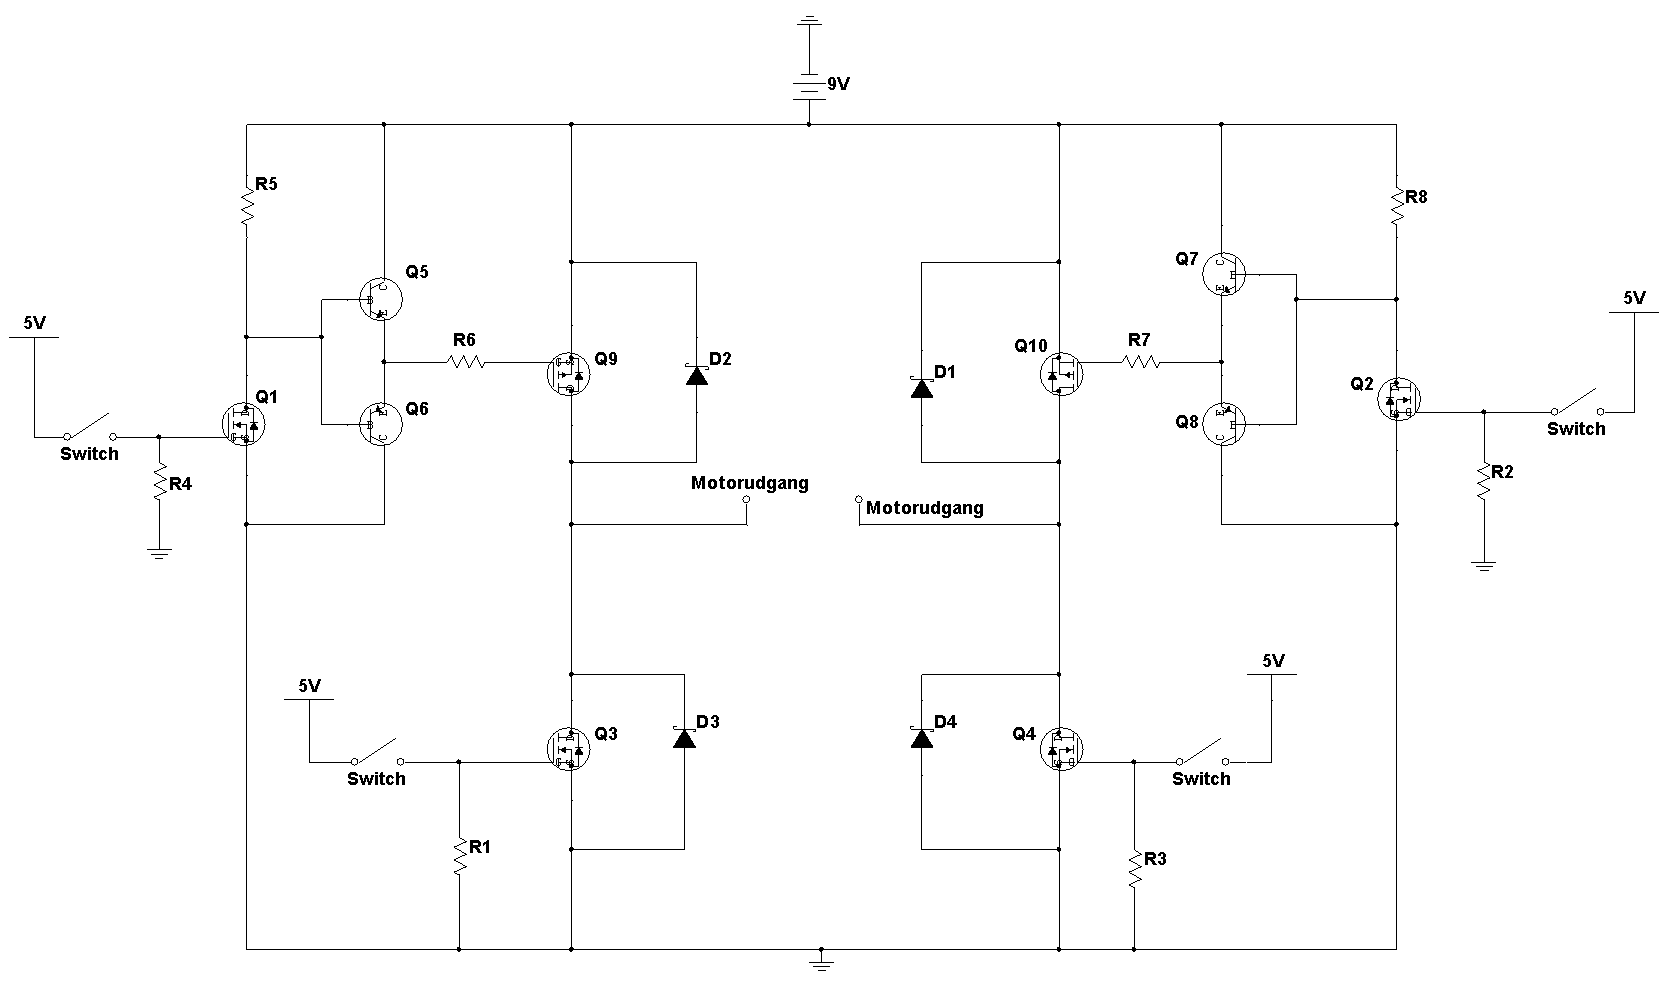
\includegraphics[width=\textwidth]{Afsnit/DesignOgImplementering/images/H-bro}
		\caption{Kredsløbsdiagram for H-broen}
		\label{fig:hbro}
\end{figure}

I tabel \ref{hbrotabel} ses relevante komponentværdier for H-broen. En fyldestgørende oversigt over disse ses i \ref{dokumentationen}

\begin{table}[H]
	\centering
	\begin{tabular}{|l|l|l}
		\cline{1-2}
		\textbf{Betegnelse} & \textbf{Komponent}  	    &  \\ \cline{1-2}
		Q1   				& IRLZ44 (MOSFET N-kanal)  	&  \\ \cline{1-2}
		Q4   				& IRLZ44 (MOSFET N-kanal)	&  \\ \cline{1-2}
		Q5   				& BC547                     &  \\ \cline{1-2}
		Q6   				& BC557                     &  \\ \cline{1-2}
		Q9   				& IRF9Z34N (MOSFET P-kanal)	&  \\ \cline{1-2}
	\end{tabular}
	\caption{Komponentbetegnelser på H-bro}
	\label{hbrotabel}
\end{table}

Når motoren skal køre fremad, skal Q9 og Q4 åbnes. For at N-MOSFET'en (Q4) kan åbne, skal der en positiv spænding ind på gatebenet. For at P-MOSFET'en (Q9) kan åbne, skal den have en negativ spænding. For at løse dette blev der sat en N-MOSFET foran hver P-MOSFET.

Da motoren gerne skal kunne skifte retning hurtigt og ofte, er det nødvendigt, at de to MOSFET's kan både åbne og lukke hurtigt. På figur \ref{fig:mof} ses, hvordan Q9 åbner og lukker langsomt, hvilket skyldes kondensatoreffekten mellem benene på MOSFET'en.

For at få Q9 til åbne hurtigere blev Q5 indsat. Der var stadig det problem, at Q9 var langsom til at lukke, og derfor blev Q6 sat ind. På figur \ref{fig:moe} ses, hvordan driveren gør, at Q9 både åbner og lukker hurtigt.

De to transistorer kunne godt have været erstattet af komponenten IRF2101, som er en driver, der gør præcis det samme, som beskrevet ovenfor. Denne er ikke anvendt, da det gav en større forståelse at udvikle driveren selv. 

\begin{figure}[H]
	\centering
	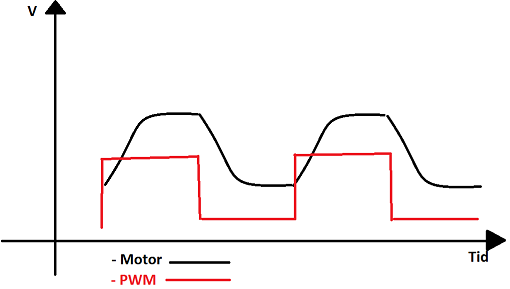
\includegraphics[width=0.3\paperwidth]{Afsnit/DesignOgImplementering/images/mof}
	\caption{Illustration af Q9's åbne- og lukketid før transistorer blev sat ind i kredsløb}
	\label{fig:mof}
\end{figure}

\begin{figure}[H]
	\centering
	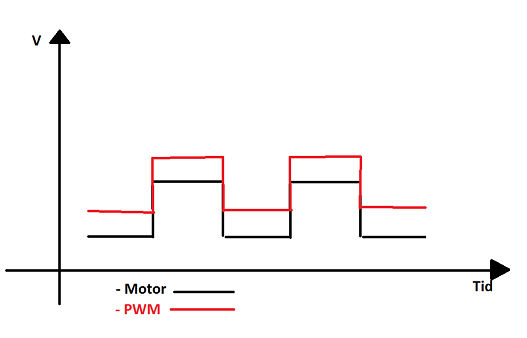
\includegraphics[width=0.3\paperwidth]{Afsnit/DesignOgImplementering/images/moe}
	\caption{Illustration af Q9's åbne- og lukketid efter transistorer blev sat ind i kredsløb}
	\label{fig:moe}
\end{figure}

De fire dioder, der er indsat i kredsløbet, skal fungere som beskyttelse af de fire MOSFET's. Det, de gør, er, at de sikrer, at den spænding, som er tilbage i motoren, når der lukkes for MOSFET'ene, ikke løber tilbage ind i mosfetene og brænder dem af.

For en fyldestgørende beskrivelse af H-broen, ses \ref{dokumentation, H-bro}. 

\subsubsection{Rotationsbegrænsning}
Platformen, som styres af motoren, må ikke kunne rotere 360 \(\deg\). Dette ses kravspecifikationen \textbf{\#ref Reference til kravspecikation (ikke-funktionelle krav)}. For at begrænse motorens bevægelse, anvendes et potentiometer samt en ADC. Når motoren bevæger sig, ændres potentiometerets modstandsværdi, og dermed ændres spændingsniveauet. På figur \ref{fig:opstillingADC} ses den endelige opstilling af rotationsbegrænsningen.

\begin{figure}[H]
	\centering
	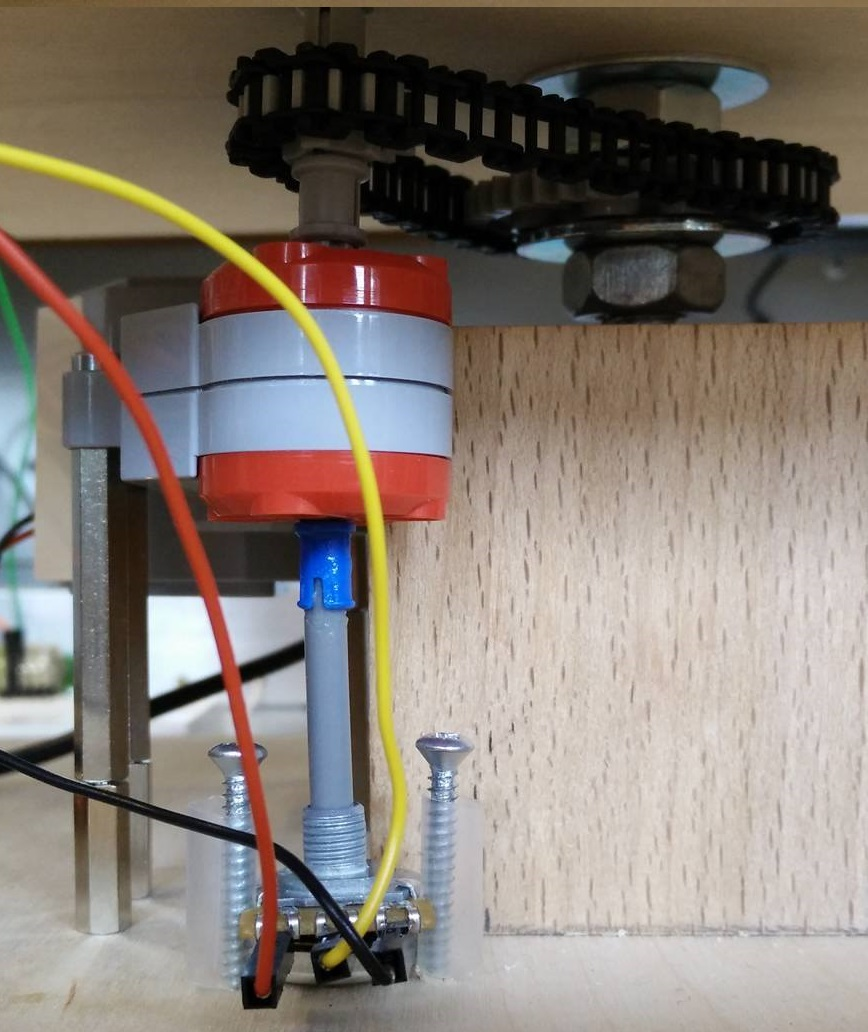
\includegraphics[scale=0.3]{Afsnit/DesignOgImplementering/images/potentiometerADC}
	\caption{Opstilling for rotationsbegrænsning}
	\label{fig:opstillingADC}
\end{figure}

\noindent \textbf{Potentiometer} \newline
Det anvendte potentiometer har en størrelse på 47\(\ K\Omega\). Denne er lineær. Det vil sige at spændingen stiger proportionalt med modstanden. I potentiometeret findes en roterende kontakt, der danner en justerbar spændingsdeler over to conceptuelle modstande. Når skaftet på potentiometret roteres ændres modstanden i de to variable modstande og dermed sker der en ændring i outputspændingen. \newline

\noindent \textbf{ADC} \newline
For at kunne aflæse spændingen på potentiometeret, anvendes en 12-bit AD converter af typen Sequencing Successive Approximation ADC. En sequencing SAR ADC indeholder et sample-hold kredsløb. Kredsløbet holder på et indgangssignal indtil det næste signal registres på kredsløbets indgang. Dermed har converteren tid til at bestemme outputværdien.


% % % % % % % % % Affyringsmekanisme % % % % % % % % % % % % % % % 
\subsection{Affyringsmekanisme}
Affyringsmekanismen består af en motor; et motorstyringskredsløb; et detektorkredsløb, der skal detektere, at motoren kun kører en enkelt omgang, når der skydes; og en kanon, som er bygget op af noget mekanik og LEGO. 

\subsubsection{Detektor}
Når kanonen affyres, styres det af motoren, og som mekanikken er opbygget, er der et propertionelt forhold mellem omdrejning på motoren og antal skud, der affyres. Derfor er det væsentligt at vide, hvornår motoren har roteret en runde, så den kan stoppes, inden der igen skydes. Til det formål anvendes detektoren. Billedet på figur \ref{fig:detektor} illustrerer hvordan detektoren anvendes.

\begin{figure}[H]
	\centering
	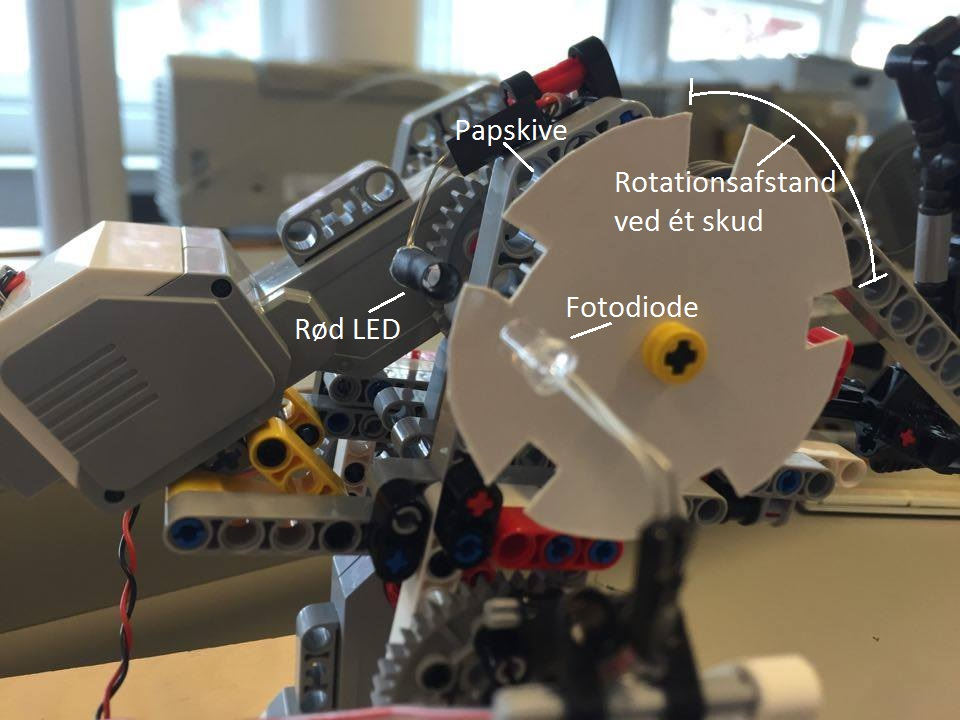
\includegraphics[width=\textwidth]{Afsnit/DesignOgImplementering/images/detektor}
	\caption{Detektorens placering på affyringsmekanismen}
	\label{fig:detektor}
\end{figure}

Den røde LED og fotodioden anbringes på affyringsmekanismen, som det ses på figur \ref{fig:detektor}. De vender ind mod hinanden, men er adskilt af papskiven. Papskiven er forbundet til motorens rotation, og hver gang et af papskivens hakker roterer forbi dioderne, kan de se hinanden. Fotodioden sender derefter et signal, som kan bruges til at stoppe motoren. Hvert hak passer med, at der er blevet affyret et skud.  

Detektoren skal kun sende et signal, når fotodioden ser lyset fra LED'en. Det er derfor vigtigt, at den ikke bliver forstyrret af dagslys og andre lyskilder. For at sikre dette, styres den røde LED af et PWM-signal, så LED'en blinker med en frekvens på 10 kHz. Detektoren opbygges tilsvarende af et båndpasfilter, med en centerfrekvens på 10 kHz, som sorterer andre frekvensområder og DC-signaler fra. 10 kHz er rigeligt højt, til at det for øjet ikke er synligt at LED'en blinker. Samtidig er det ikke for højt til, at en almindelig operationsforstærker kan håndtere det. På figur \ref*{fig:detektortand} ses et kredsløbsdiagram for detektoren og LED'en.

\begin{figure}[H]
	\centering
	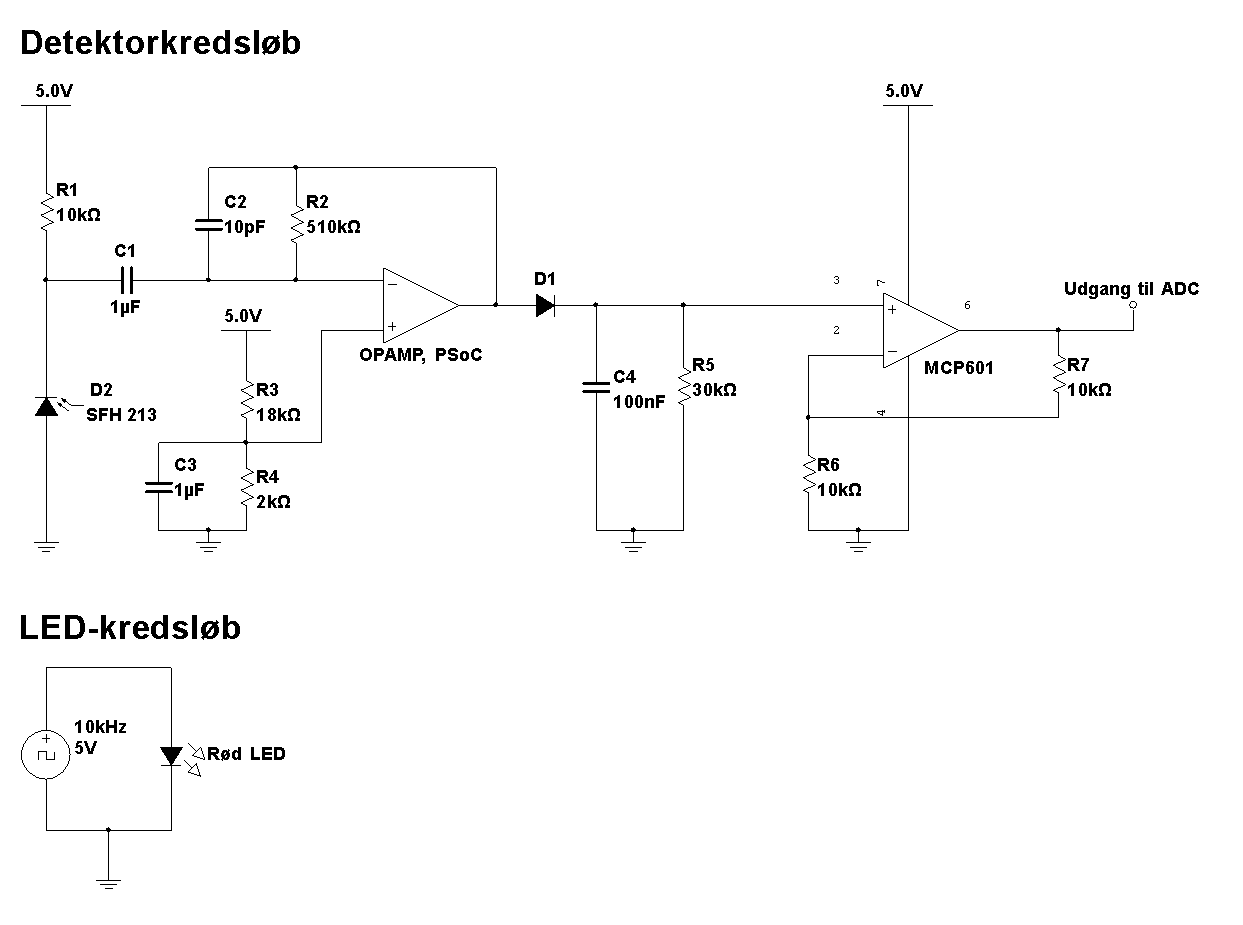
\includegraphics[width=\textwidth]{Afsnit/DesignOgImplementering/images/detektor_tandhjul}
	\caption{Kredsløbsdiagram for detektoren}
	\label{fig:detektortand}
\end{figure}


\subsubsection{Motorstyring}
Til at styre affyringsmekanismens motor er der bygget et kredsløb med en MOSFET som primære komponent. MOSFET'en skal sørge for, at motoren kun kører, når der bliver sendt PWM-signal ind i den. Kredsløbsdiagrammet kan ses på figur \ref{fig:affyringsmotor}. 

\begin{figure}[H]
	\centering
	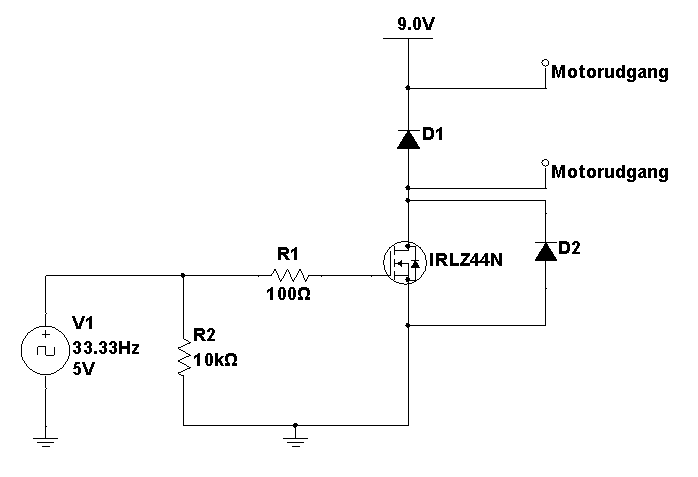
\includegraphics[width=0.7\textwidth]{Afsnit/DesignOgImplementering/images/affyringsmotor}
	\caption{Diagram over motorstyring til motor på affyringsmekanisme}
	\label{fig:affyringsmotor}
\end{figure}

Dioden D1 er sat ind for at sikre motoren mod store spændingsspikes, der kan forekomme, når MOSFET'en bliver afbrudt. Dioden D2, der sidder fra source til drain, sikrer, at spikes genereret af motoren, når den slukkes, ikke brænder MOSFET'en af. 

\subsubsection{Kanon og platform}
Selve kanonen og platformen den står på er bygget op af to træplader og LEGO. Den ene træplade kan dreje fra side til side, således at det er muligt at sigte i den horisontale retning. Opbygningen ses på figur \ref{fig:Horisontalmekanik}. Træpladen placeres på den øverste metalskive omkring skruen, så den drejer med rundt, når motoren roterer. Rotationen er opnået ved, at skruen kan dreje frit, men stadig er holdt lodret. Det store tandhjul er boret ud i midten, og der er indsat en møtrik, så den kan skrues på skruen. Forholdet mellem det store og det lille tandhjul gør at rotationshastigheden bliver gearet ned. Endeligt er motoren skruet fast til den nederste træplade, men i en højde, der gør at den kan drive det lille tandhjul, som er forbundet med gearkæden til det store tandhjul. 

\begin{figure}[H]
	\centering
	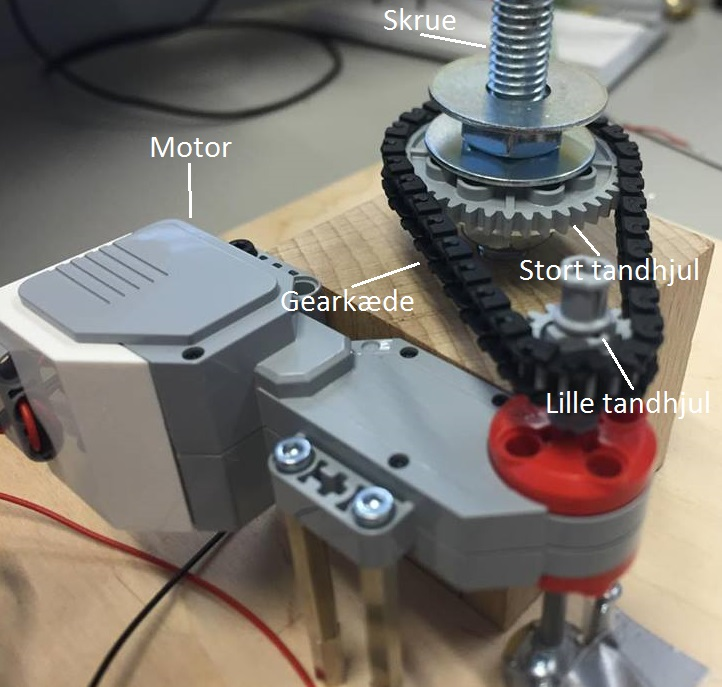
\includegraphics[width=1\textwidth]{Afsnit/DesignOgImplementering/images/horisontalMekanik}
	\caption{Horisontal mekanik}
	\label{fig:Horisontalmekanik}
\end{figure}

Mekanikken for den vertikale retning er bygget af LEGO. Et billede af opbygningen ses på figur \ref{fig:kanon}. Styringen af den vertikale bevægelse bliver håndteret af den vertikale motor, som ses på figur \ref{fig:kanon}. Motoren er forbundet til tandhjulene til vertikal styring. Der er ét tandhjul på hver side af motoren. De er begge bygget sammen med resten af kanonen. Når motoren drejer, bliver tandhjulene og hele kanonen vippet fremover eller bagover. 

Ligesom den vertikale styring er selve kanonen også bygget i LEGO. Den har et magasin, som det fremgår af figur \ref{fig:kanon}. Der kan kommes slik i magasinet, som så bliver affyret. Affyringen styres af den anden motor på figur \ref{fig:kanon}. Når affyringsmotoren drejer bliver to større tandhjul roteret. De to tandhjul er desuden forbundet til to små tandhjul, som er 5 gange så små. Med denne gearing roterer de små tandhjul 5 gange så hurtigt. De små tandhjul er forbundet til to mellem størrelse tandhjul, som drejer med dem rundt. Tandhjulene i mellemstørrelse styrer affyringen ved at omdanne den roterende bevægelse til en vandret bevægelse frem og tilbage, som affyrer kanonen.

\begin{figure}[H]
	\centering
	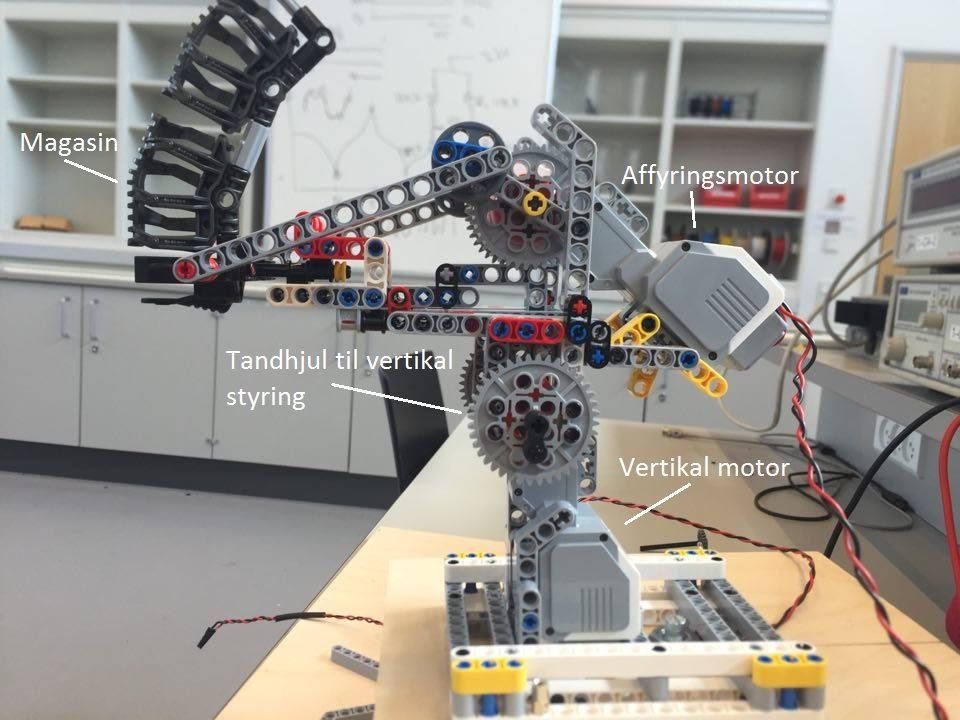
\includegraphics[width=1\textwidth]{Afsnit/DesignOgImplementering/images/kanon}
	\caption{Kanon i LEGO}
	\label{fig:kanon}
\end{figure}
 

\section{Software}

\subsection{SPI - Devkit8000}
candygun-driveren sørger for SPI-kommunikationen fra Devkit8000 til PSoC0. Driveren er skrevet i c, hvilket er typisk for drivere til linuxplatforme. I forbindelse med design og implementering af SPI, er der nogle indstillinger, der skal vælges. Disse indstilligner ses på tabel \ref{SPItabel}. Yderligere uddybning af de forskellige indstillinger kan ses i dokumentationen \#ref 

\begin{table}[H]
	\centering
	\caption{Indstillinger for SPI}
	\label{SPItabel}
	\begin{tabular}{|l|l|}
		\hline
		\textbf{Indstillingsparameter} & \textbf{Værdi} \\ \hline
		SPI bus nr.                    & 1              \\ \hline
		SPI chip-select                & 0              \\ \hline
		Hastighed                      & 1 MHz          \\ \hline
		SPI Clock Mode                 & 3              \\ \hline
		Bit per transmission           & 8              \\ \hline
	\end{tabular}
\end{table}

%SPI-kommunikationen er implementeret med SPI bus nummer 1, SPI chip-select 0 og en hastighed på 1 MHz (et godt stykke under max på 20 MHz for en sikkerhedsskyld). Desuden starter clocken højt og data ændres på falling edge og aflæses på rising edge. Dermed bliver SPI Clock Mode 3. Derudover sendes der 8 bit pr transmission, hvilket passer med SPI-protokollen for projektet.\\
%For at kunne anvende driveren, når SPI er tilsluttet, er der oprettet et hotplugmodul, som fortæller kernen, at der er et SPI device, som matcher driveren. Det kan SPI-forbindelsen ikke selv gøre, som usb fx kan.  

Selve driveren er i filen candygun.c opbygget som en char driver. For at holde forskellige funktionaliteter adskilt, er alle funktioner, der har med SPI at gøre, implementeret i filen candygun-spi.c.  På figur \ref{fig:spiklasse} ses et klassediagram for opbygningen af driveren. I programmeringssproget c findes der ikke klasser, men selvom filerne i driveren ikke er opbygget som klasser, er de repræsenteret sådan i diagrammet for overskuelighedensskyld. De stiplede linjer i diagrammet indikerer at den ene klasse anvender den andens motoder, på samme måde som ved et bibliotek. spi.h, som også ses i diagrammet, er en indbygget del Linux, og er derfor ikke yderligere dokumenteret her. 

\begin{figure}[H]
	\centering
	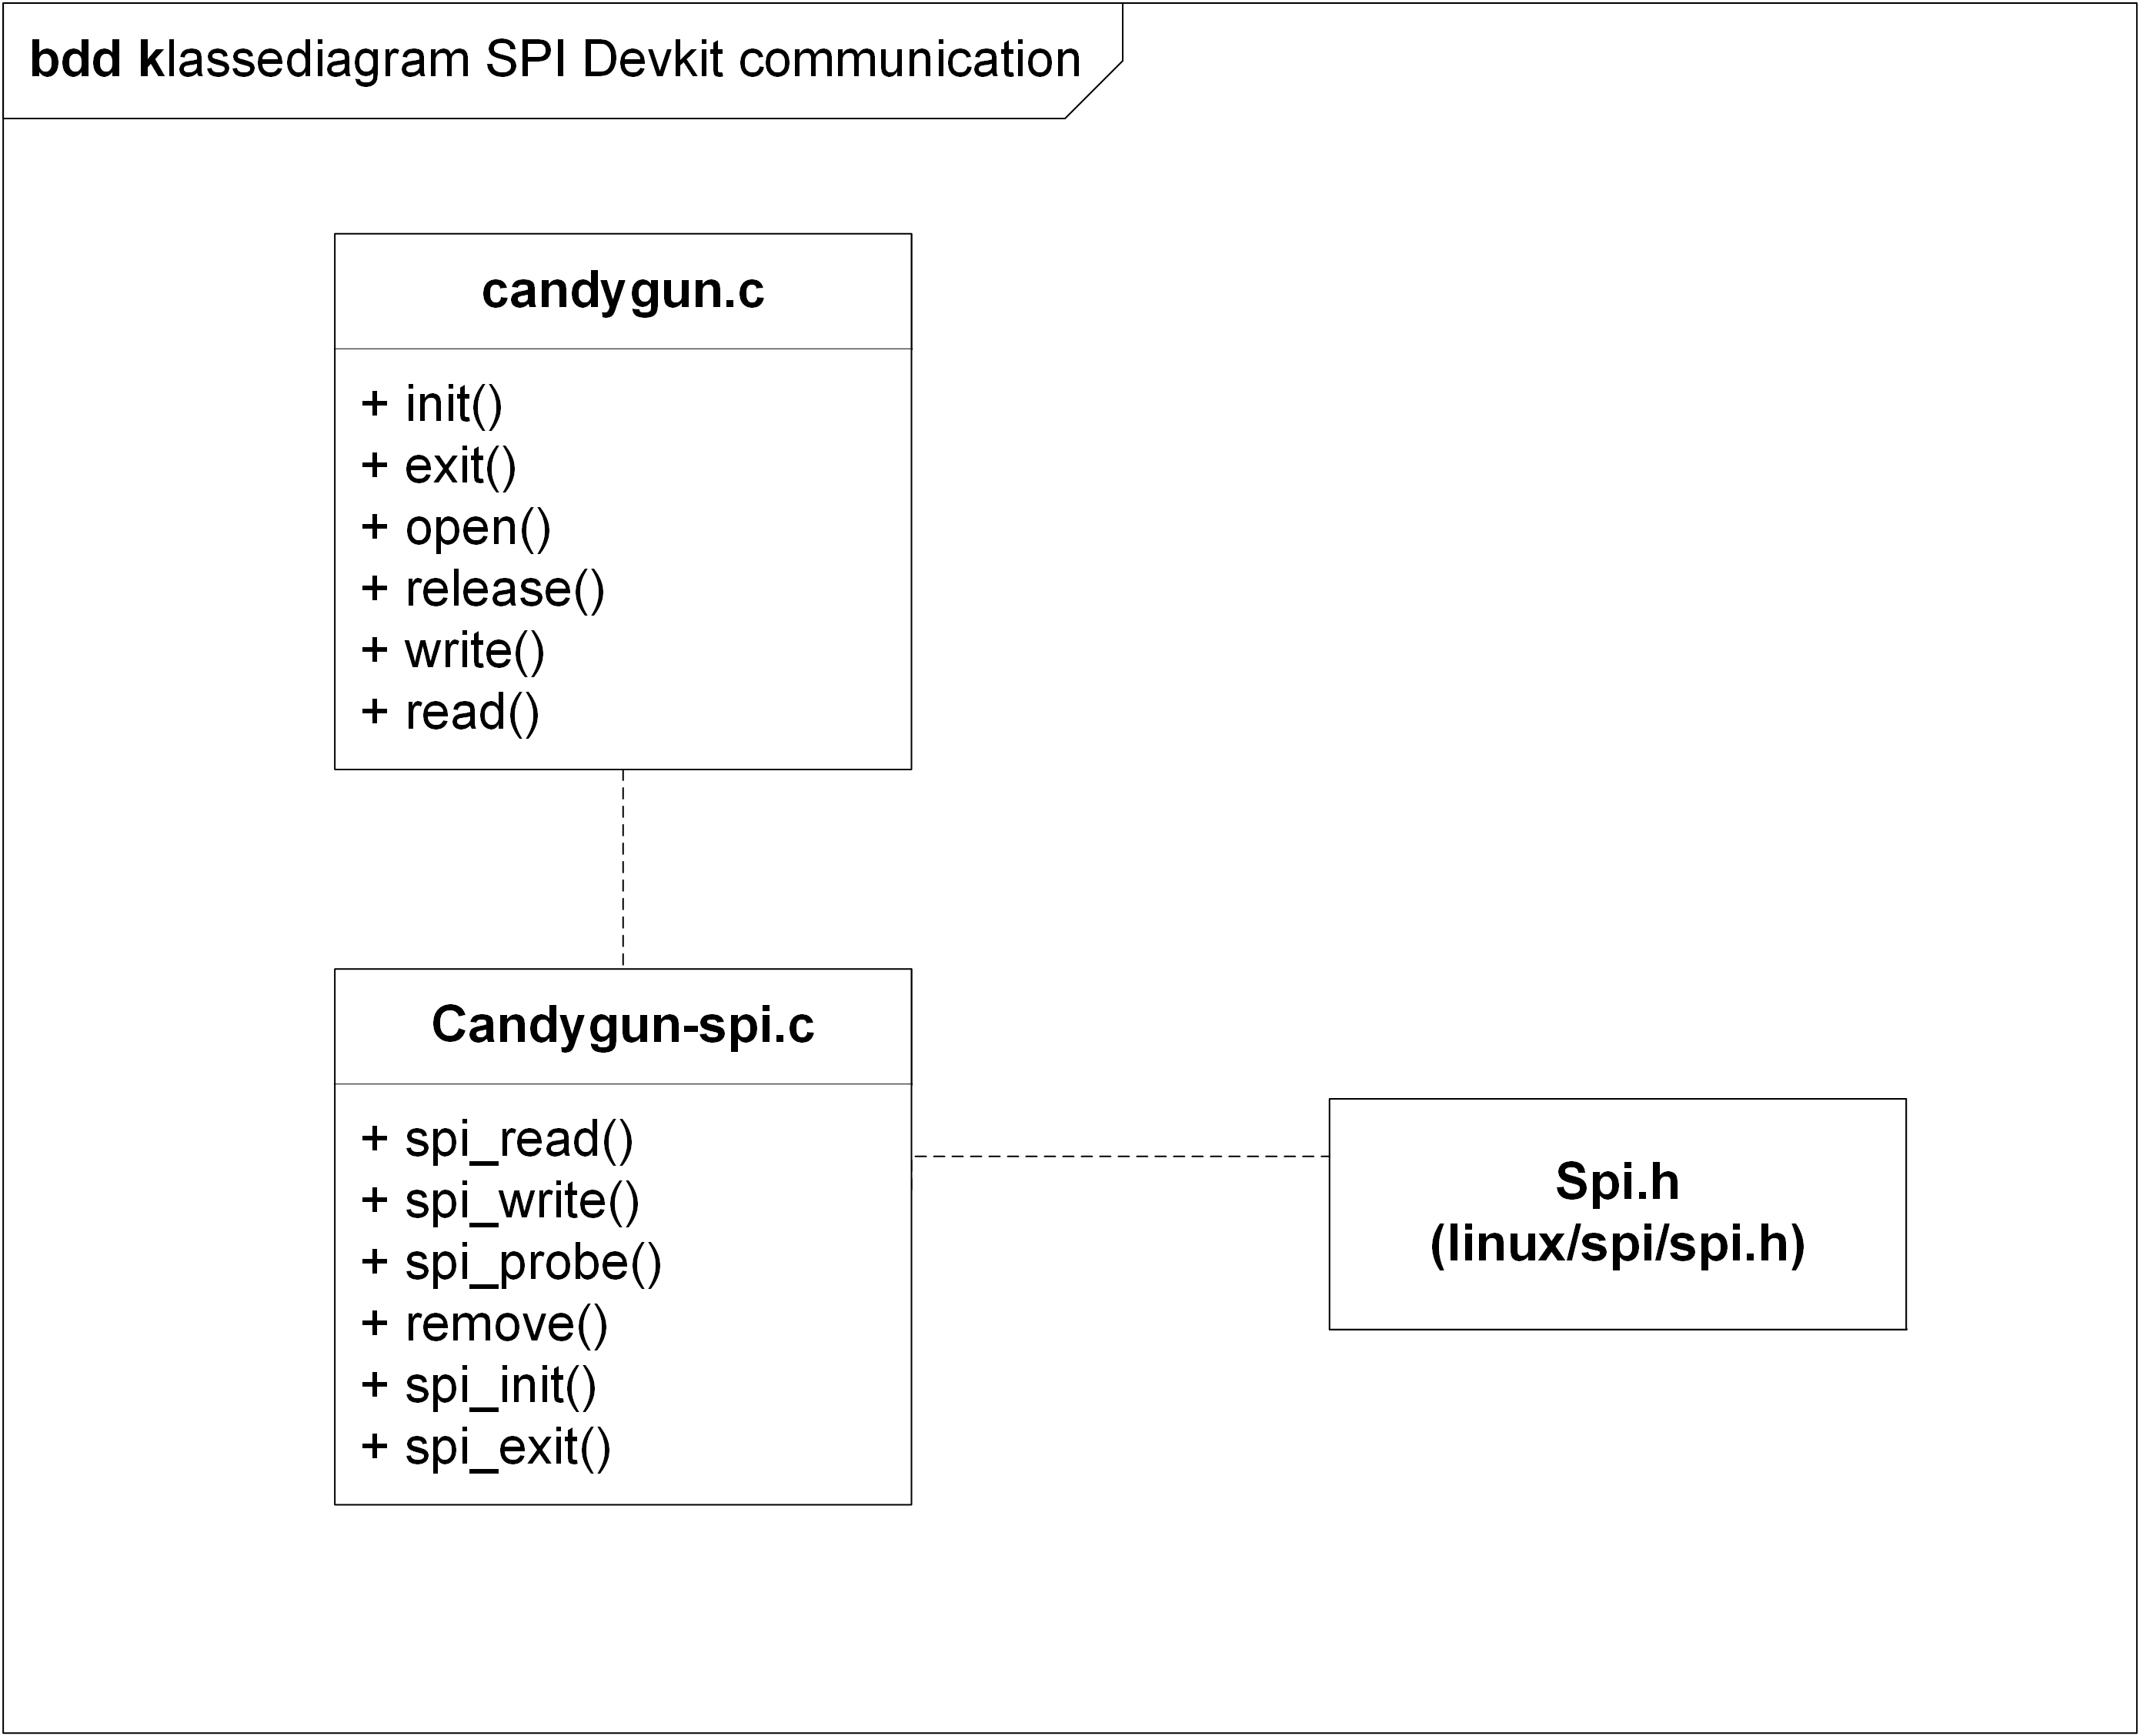
\includegraphics[width=\textwidth]{Afsnit/DesignOgImplementering/images/SPIklasse}
	\caption{Klassediagram for SPI kommunikation på Devkit 8000}
	\label{fig:spiklasse}
\end{figure}

%I probe-funktionen sættes bits\textunderscore per\textunderscore word til 8, da vi sender otte bit som nævnt tidligere. I exit-funktionen anvender candygun.c igen en funktion fra candygun-spi.c - denne gang til at frigive SPI ressourcen. Når der fx skal requestes en SPI ressource i init-funktionen i candygun.c, så anvender driveren en funktion fra candygun-spi.c til det.
% I write-metoden gives der data med fra brugeren. I dette tilfælde udgøres brugeren af Interface driveren og dataet er en 8 bit kommando fra SPI-protokollen. Dog er dataet fra brugeren i første omgang læst ind som en charstreng. I write-metoden bliver det så lavet om til en int.  For at overføre dataet på en sikker måde anvendes funktionen copy\textunderscore from\textunderscore user() til at overføre data fra brugeren. Write-funktionen fra candygun.c anvender derefter en write-funktion fra candygun-spi.c, hvor den sender brugerinputtet med. I den spi-relaterede write-funktion bliver bruger inputtet lagt i transfer bufferen og der NULL bliver lagt i receive bufferen, og med spi\textunderscore sync-funktionen bliver det sendt.\\ 
Når der skal skrives og læses, anvendes read- og write-funktionerne. Ofte ville en spi read-funktion først indeholde en write-del, som fortalte SPI-slaven, hvad der skulle læses over i bufferen. Det ville typisk efterfølges af et delay og så en read-del. Men i dette projekt skal der ofte afventes et brugerinput, som ikke kan styres af et fast delay, og der er generelt et behov for at sende en aktiv kommando, før der læses. Derfor er det besluttet at read-funktionen kun indeholder en read-del i transmissionen. Dermed skal write-funktionen altid aktivt anvendes inden der læses, da PSoC0 ellers ikke ved, hvad der skal gøres/lægges i bufferen. De resterende metoder, som ses i klassediagrammet på figur \ref{fig:spiklasse}, er uddybet i dokumentationen \#ref.\\
% Når funktionen har modtaget resultatet fra transmissionen returneres det til brugeren med funktionen copy\textunderscore to\textunderscore user(), som igen sørger for at overførslen af data foregår på en sikker måde.
   
\subsection{Brugergrænseflade}
I det følgende afsnit bliver delene i den overordenede brugergrænseflade beskrevet.

\subsubsection{Interface Driver}
Interface driveren fungerer som bindeled mellem brugergrænsefladen og candydriveren på Devkit8000. Den indeholder tre funktioner.

\begin{figure}[H]
	\centering
	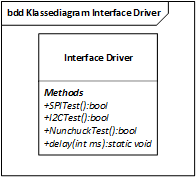
\includegraphics[width=0.5\textwidth]{Afsnit/DesignOgImplementering/images/InterfacedriverKlassediagram}
	\caption{Klassediagram for Interfacedriver}
	\label{fig:idriverclass}
\end{figure}

Interface driveren indeholder fire metoder: SPITest(), I2CTest(), NunchuckTest() og delay(int ms). De tre test metoder anvendes til at starte en test af de forskellige kommunikationsforbindelser: SPI, I2C og Nunchuck forbindelse.
Hver af disse tre metoder tilgår /dev/candygun på DevKit8000.
De skriver en unik værdi til filen, som SPI-driveren tilgår.
Efter hver tilskrivning lukkes adgangen til filen. Herefter kaldes delay-metoden, så andre dele af systemet har tid til at skrive et svar til /dev/candygun. Herefter læser metoderne fra filen. Rækkefølgen for metodekaldende kan ses på figur \ref{fig:SystemTestSekvensDiagram}

\subsubsection{Systemtest GUI}
\label{afsnit:sysGUI}
Usecase 2 styres via Systemtest GUI'en fra Devkit8000.
Dette afsnit beskriver Systemtest GUI'ens design. Figur \ref{fig:GUIPic} viser GUI'en for use case 2.

\begin{figure}[H]
	\centering
	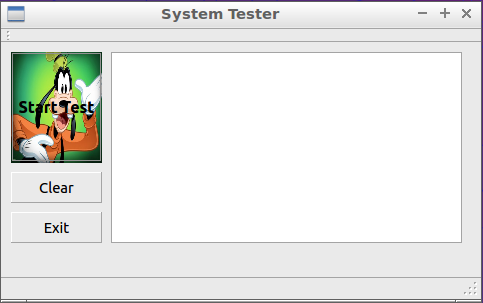
\includegraphics[width=\textwidth]{Afsnit/DesignOgImplementering/images/GUIPic}
	\caption{Brugergrænseflade for usecase 2 - Test kommunikationsprotokoller}
	\label{fig:GUIPic}
\end{figure}

Systemtest GUI'en er lavet med det indbyggede design framework i QT Creator 5\cite{Website:QTCreator}, se dokumentation \#refDokuUdvikling.
QT frameworket opretter "hovedvinduet" i GUI'en som en klasse. Knapperne tilføjes som private slots i klassen
hvilket gør dem i stand til interagere i GUI'en. Når en knap er assignet til et slot i klassen, og der trykkes på den pågældende knap, bliver det tildelte signal broadcastet
og slot-funktionen bliver kørt. Alle tre knapper i GUI'en er assignet signal-typen "clicked()".

Her vises en statemachine for Systemtest GUI'ens forløb igennem usecase 2.

\begin{figure}[H]
	\centering
	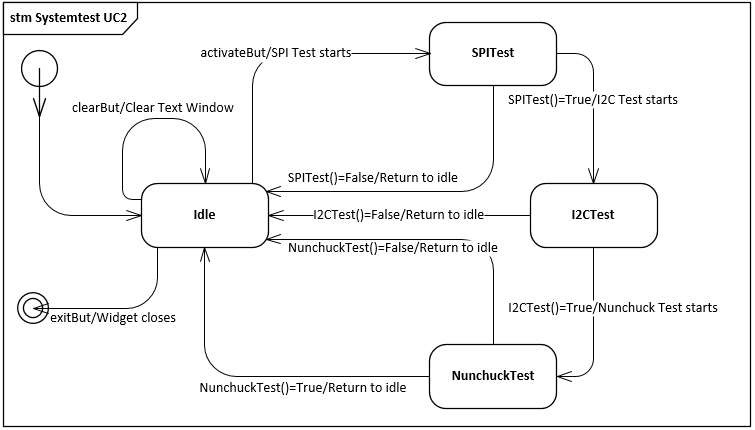
\includegraphics[width=1.2\textwidth]{Afsnit/DesignOgImplementering/images/StateMachineUC2}
	\caption{State machine for Systemtest GUI}
	\label{fig:StateMachineUC2}
\end{figure}

Statemachinens, figur \ref{fig:StateMachineUC2}, forløb beskrives i dokumentationen, \#RefDoku

Systemtest GUI'en for UC2 er en simpel test-konsol. Den består af 3 knapper og et konsol vindue. GUI'en interfacer med SPI-protokollen, gennem vores interface driver. Den første knap, Start test, initierer UC2. Efterhånden som testen løbes igennem kaldes test funktionerne, og ved hjælp af if-conditions, bliver der tjekket på retur-værdierne fra interface-funktionerne. Hvis retur-værdien er true, skrives der en "--test successful" besked i konsol vinduet. og widgeten kører videre. Hvis retur-værdien er false, skrives der en "--test unsuccessful" i tekstvinduet og GUI'en returnerer til idle tilstand. Når alle test er successful, skrives "System test successful, system is ready for use" til konsol vinduet, og GUI'en returnerer til idle tilstand. Den anden knap, Clear, clearer konsollen til blank tilstand. Den tredje knap, Exit, lukker GUI'en.
Koblingen i GUI'en hænger udelukkende sammen med interfacedriveren. Knapperne kalder funktioner fra interfacedriveren, og ved ændring i disse funktioner, ville foresage ændringer i GUI'en.

\subsubsection{Demo GUI}

I dette afsnit beskriver Demo GUI'en for usecase 1.
Strukturen for denne GUI er lignende til Systemtest GUI'en.
Denne demo er en repræsentation af hvad der kunne være en færdig implementeret
GUI til usecase 1.

\begin{figure}[H]
	\centering
	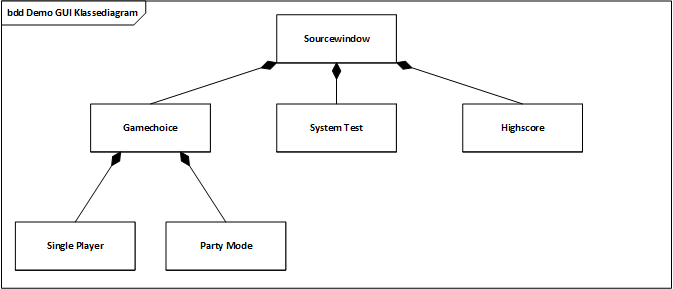
\includegraphics[width=1.2\textwidth]{Afsnit/DesignOgImplementering/images/DemoGUIClass}
	\caption{Klassediagram for Demo GUI}
	\label{fig:DemoGUIClass}
\end{figure}

Demo'en består af seks vinduer, hvert vindue har en tilhørende klasse, se figur \ref{fig:DemoGUIClass}.
Hovedvinduet har klassen sourcewindow. Sourcewindow består af fire knapper,
hvor tre af dem åbner nye vinduer og den fjerde lukker GUI'en.
De tre vinduer der kan åbnes fra sourcewindow er: Gamechoice, Highscore, og System Test.
Highscore vinduet består af tre knapper og et konsol vindue. System Test er Systemtest Gui'en
implementeret i Demo GUI'en, se afsnit \ref{afsnit:sysGUI} for detajler.
Gamechoice består af tre knapper. To af knapper åbner to nye vinduer og den tredje knap lukker vinduet
og returnerer programmet til sourcewindow. De to vinduer åbnes er Single Player og Party Mode.
Single player består af et konsol vindue og en exit-knap, Party mode består af to konsol vinduer og en exit-knap.


\begin{figure}[H]
	\centering
	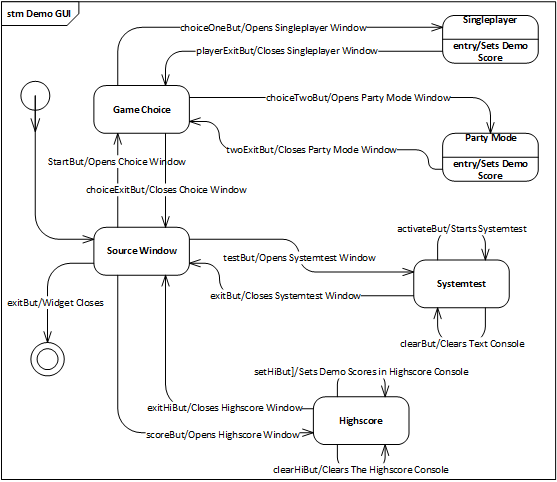
\includegraphics[width=1.2\textwidth]{Afsnit/DesignOgImplementering/images/StateMachineDemoGUI}
	\caption{State machine for Demo GUI}
	\label{fig:StateMachineDemo}
\end{figure}

State Machinen, figur \ref{fig:StateMachineDemo}, forklarer, hvordan Demo GUI'ens vinduer skifter tilstand i forhold til event-triggers.
\#RefDokuStatemachineforklaring

\subsection{Nunchuck}
Til styring af kanonen bruges en Wii-nunchuck. Følgende afsnit beskriver PSoC0's håndtering af data fra Wii-nunchuck.

\subsubsection{Afkodning af Wii-Nunchuck Data Bytes}
Aflæste bytes fra Wii-Nunchuck - indeholdende tilstanden af knapperne og det analoge stick - er kodet når de oprindeligt modtages via I2C bussen. Disse bytes skal altså afkodes før deres værdier er brugbare. Afkodningen af hver byte sker ved brug af følgende formel:

\textit{AfkodetByte = (AflæstByte XOR 0x17) + 0x17}

Fra formlen kan det ses at den aflæste byte skal \textit{XOR}'s (Exclusive Or) med værdien 0x17, hvorefter dette resultat skal adderes med værdien 0x17.

\subsubsection{Kalibrering af Wii-Nunchuck Analog Stick}
De afkodede bytes for Wii-Nunchuck's analoge stick har definerede standardværdier for dets forskellige fysiske positioner. Disse værdier findes i tabel \ref{tabel:WiiNunchuckStickPositioner}

\begin{table}[H]
	\centering
	\begin{tabular}{|l|l|}
		\hline
		X-akse helt til venstre & 0x1E \\ \hline
		X-akse helt til højre   & 0xE1 \\ \hline
		X-akse centreret        & 0x7E \\ \hline
		Y-akse centreret        & 0x7B \\ \hline
		Y-akse helt frem        & 0x1D \\ \hline
		Y-akse helt tilbage     & 0xDF \\ \hline
	\end{tabular}
	\caption{Standardværdier for fysiske positioner af Wii-Nunchuck's analoge stick}
	\label{tabel:WiiNunchuckStickPositioner}
\end{table}

I praksis skal de afkodede værdier for det analoge stick kalibreres, da slør pga. brug gør at de ideale værdier ikke rammes. 

I projektet er de afkodede værdier for det analoge stick kalibreret med værdien -15 (0x0F i hexadecimal), altså ser den endelige formel for afkodning samt kalibrering således ud:

\textit{AfkodetByte = (AflæstByte XOR 0x17) + 0x17 - 0x0F}

\subsection{PSoC Software}
På figur \ref{figure:klassediagramPSoC0} og \ref{figure:klassediagramPSoC1} ses de endelige klassediagrammer for PSoC0 og PSoC1. Disse klassediagrammer er designet ud fra applikationsmodellerne i dokumentationen \textbf{\#ref Reference til applikationsmodeller i dokumentatonen} og de samlede klassediagrammer for UC1- og 2 i systemarkitekturen figur \ref{fig:CompleteClassDiagramPSoC0} og \ref{fig:CompleteClassDiagramPSoC1}. For at opretholde høj samhørighed, er der lavet en klasse for hver grænseflade. F.eks. indeholder "Nunchuck"-klassen al den software der skal til for at kommunikere med en nunchuck-enhed. 

De efterfølgende afsnit vil beskrive klasserne og deres funktioner.

\begin{figure}[H]
	\begin{adjustwidth}{-2cm}{-\rightmargin}
		\centering
		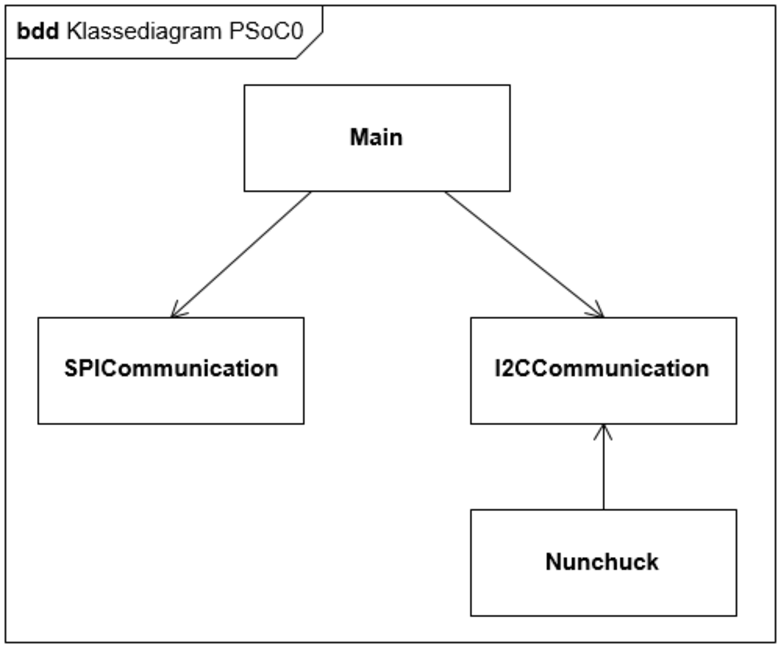
\includegraphics[width=1.35\textwidth]{DesignOgImplementering/images/PSoC0KlassediagramOversigt.pdf}
		\caption{Klassediagram for PSoC0}
		\label{figure:klassediagramPSoC0}
	\end{adjustwidth}
\end{figure}

\begin{figure}[H]
	\centering
	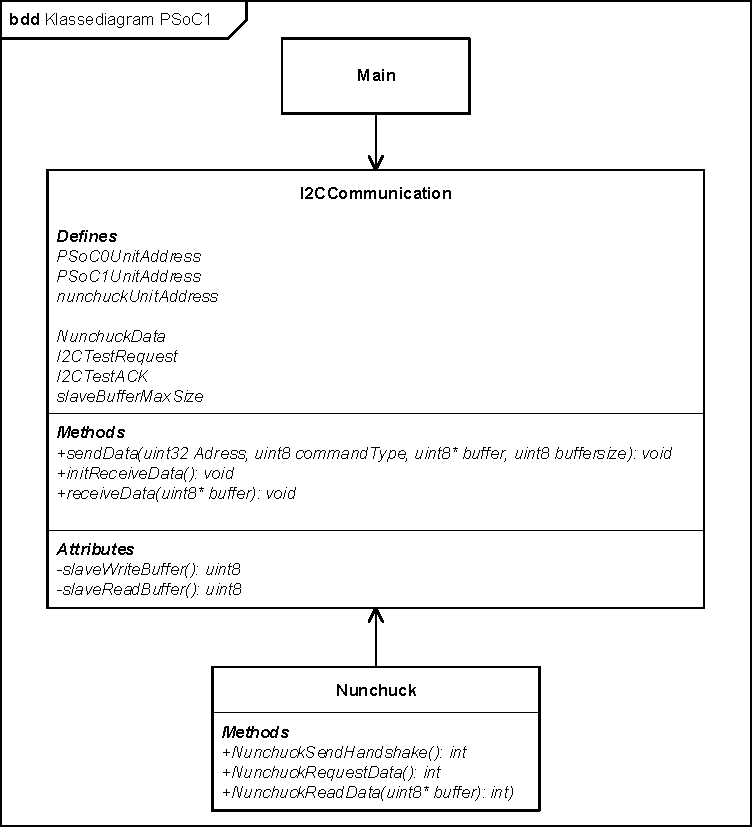
\includegraphics[width=\textwidth]{DesignOgImplementering/images/PSoC1KlassediagramOversigt.pdf}
	\caption{Klassediagram for PSoC1}
	\label{figure:klassediagramPSoC1}
\end{figure}

\subsubsection{I2CCommunication}
I systemarkitekturen på figur \ref{fig:CompleteClassDiagramPSoC0} og \ref{fig:CompleteClassDiagramPSoC1}, er der udarbejdet klassediagrammer der beskriver funktionaliteterne for PSoC0- og 1 softwaren. Mht. til I2C-kommunikation klassen, er den overordnede funktionalitet, at kunne sende og modtage data via I2C-nettet. På figur \ref{figure:klassediagramI2CCommunication} ses klassediagrammet for I2CCommunication klassen, der netop har metoder og attributter til at dække disse behov.


\begin{figure}[H]
	\centering
	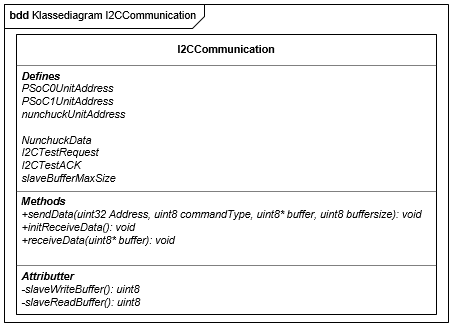
\includegraphics[]{DesignOgImplementering/images/I2CCommunication}
	\caption{Klassediagram for I2CCommunication klassen}
	\label{figure:klassediagramI2CCommunication}
\end{figure}

Den fulde klassebeskrivelse for I2CCommunication klassen kan findes i dokumentationen \#ref \textbf{Indsæt reference til klassebeskrivelse for I2CCommunication i dokumentationen}.

\subsubsection{Nunchuck}
Nunchuck klassen er seperat fra I2CCommunication klassen, på trods af at kommunikationen foregår over I2C-bussen, idét at Nunchucken bruger sin egen kommunikationsprotokol, som defineret i \#ref \textbf{Reference til nunchuck i bilag}. Fra figur \ref{fig:CompleteClassDiagramPSoC0} og \ref{fig:CompleteClassDiagramPSoC1} i systemarkitekturen der omhandler PSoC software, er det udledt at softwaren skal have metoder til at skrive og læse fra nunchucken. På figur \ref{figure:NunchuckKlassediagram} ses klassediagrammet for den implementerede nunchuck klasse, der indeholder metoder der har disse funktionaliteter.


\begin{figure}[H]
	\centering
	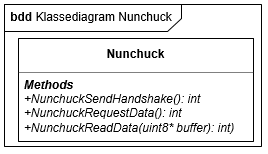
\includegraphics[]{DesignOgImplementering/images/nunchuck}
	\caption{Klassediagram for klassen Nunchuck}
	\label{figure:NunchuckKlassediagram}
\end{figure}

Den fulde klassebeskrivelse for Nunchuck klassen og dens metoder kan ses i dokumentationen side \#ref \textbf{Reference til Nunchuck klassebeskrivelser i dokumentationen} 

\subsubsection{SPI - PSoC}
I dette afsnit vil softwaren der specifikt omhandler SPI-kommunikationen mellem PSoC0 og DevKit8000 blive beskrevet fra PSoC-CPU'ens perspektiv. På figur \ref{figure:KlassediagramSPICommunication} ses den klasse der omhandler SPI-kommunikationen i systemet. Ud fra klassediagrammet figur \ref{fig:CompleteClassDiagramPSoC0} i systemarkitekturen, er det blevet udledt at SPI-klassen skal kunne starte og gennemføre forskellige test. Figur \ref{figure:KlassediagramSPICommunication} viser klassediagrammet for den implementerede klasse, der afspejler netop dette.


\begin{figure}[H]
	\centering
	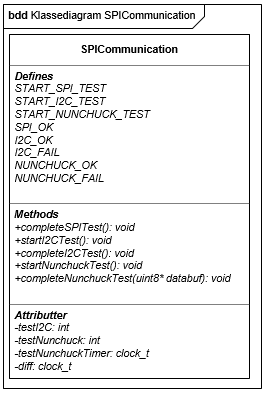
\includegraphics[]{DesignOgImplementering/images/SPICommunication}
	\caption{Klassediagram over klassen SPICommunication}
	\label{figure:KlassediagramSPICommunication}
\end{figure}

En detaljeret klassebeskrivelse for SPICommunication klassen kan findes i dokumentationen side \#ref \textbf{Referer til SPICommunication klassebeskrivelse i dokumentationen}.

\subsection{PSoC2 - Affyringsmekanisme}
 
Affyringsmekanismen består udover hardware og mekanik også flere softwaredele, som er programmeret på PSoC2. Til rotationsdetektorens operationsforstærker er der anvendt en, der er indbygget i PSoC'en. Derudover styres bl.a. interrupt og PWM-signaler i forbindelse med affyringsmekanismen ved hjælp af PSoC2. Desuden aflæses spændingen fra rotationsdetektoren af en SAR ADC, som også findes på PSoC2. For at se hvor de forskellige pins er ført ud til på PSoC2, og yderligere uddybning af indstillingerne for de forskellige blokke henvises til dokumentationen \ref{Dokumentation PSoC2 sofware}. I forbindelse med affyringen af kanonen køres en kodesekvens. Et sekvensdiagram for afviklingen af koden ses på figur \ref{fig:aktivitetsdiagramDetektor}. 
 
\begin{figure}[H]
	\centering
	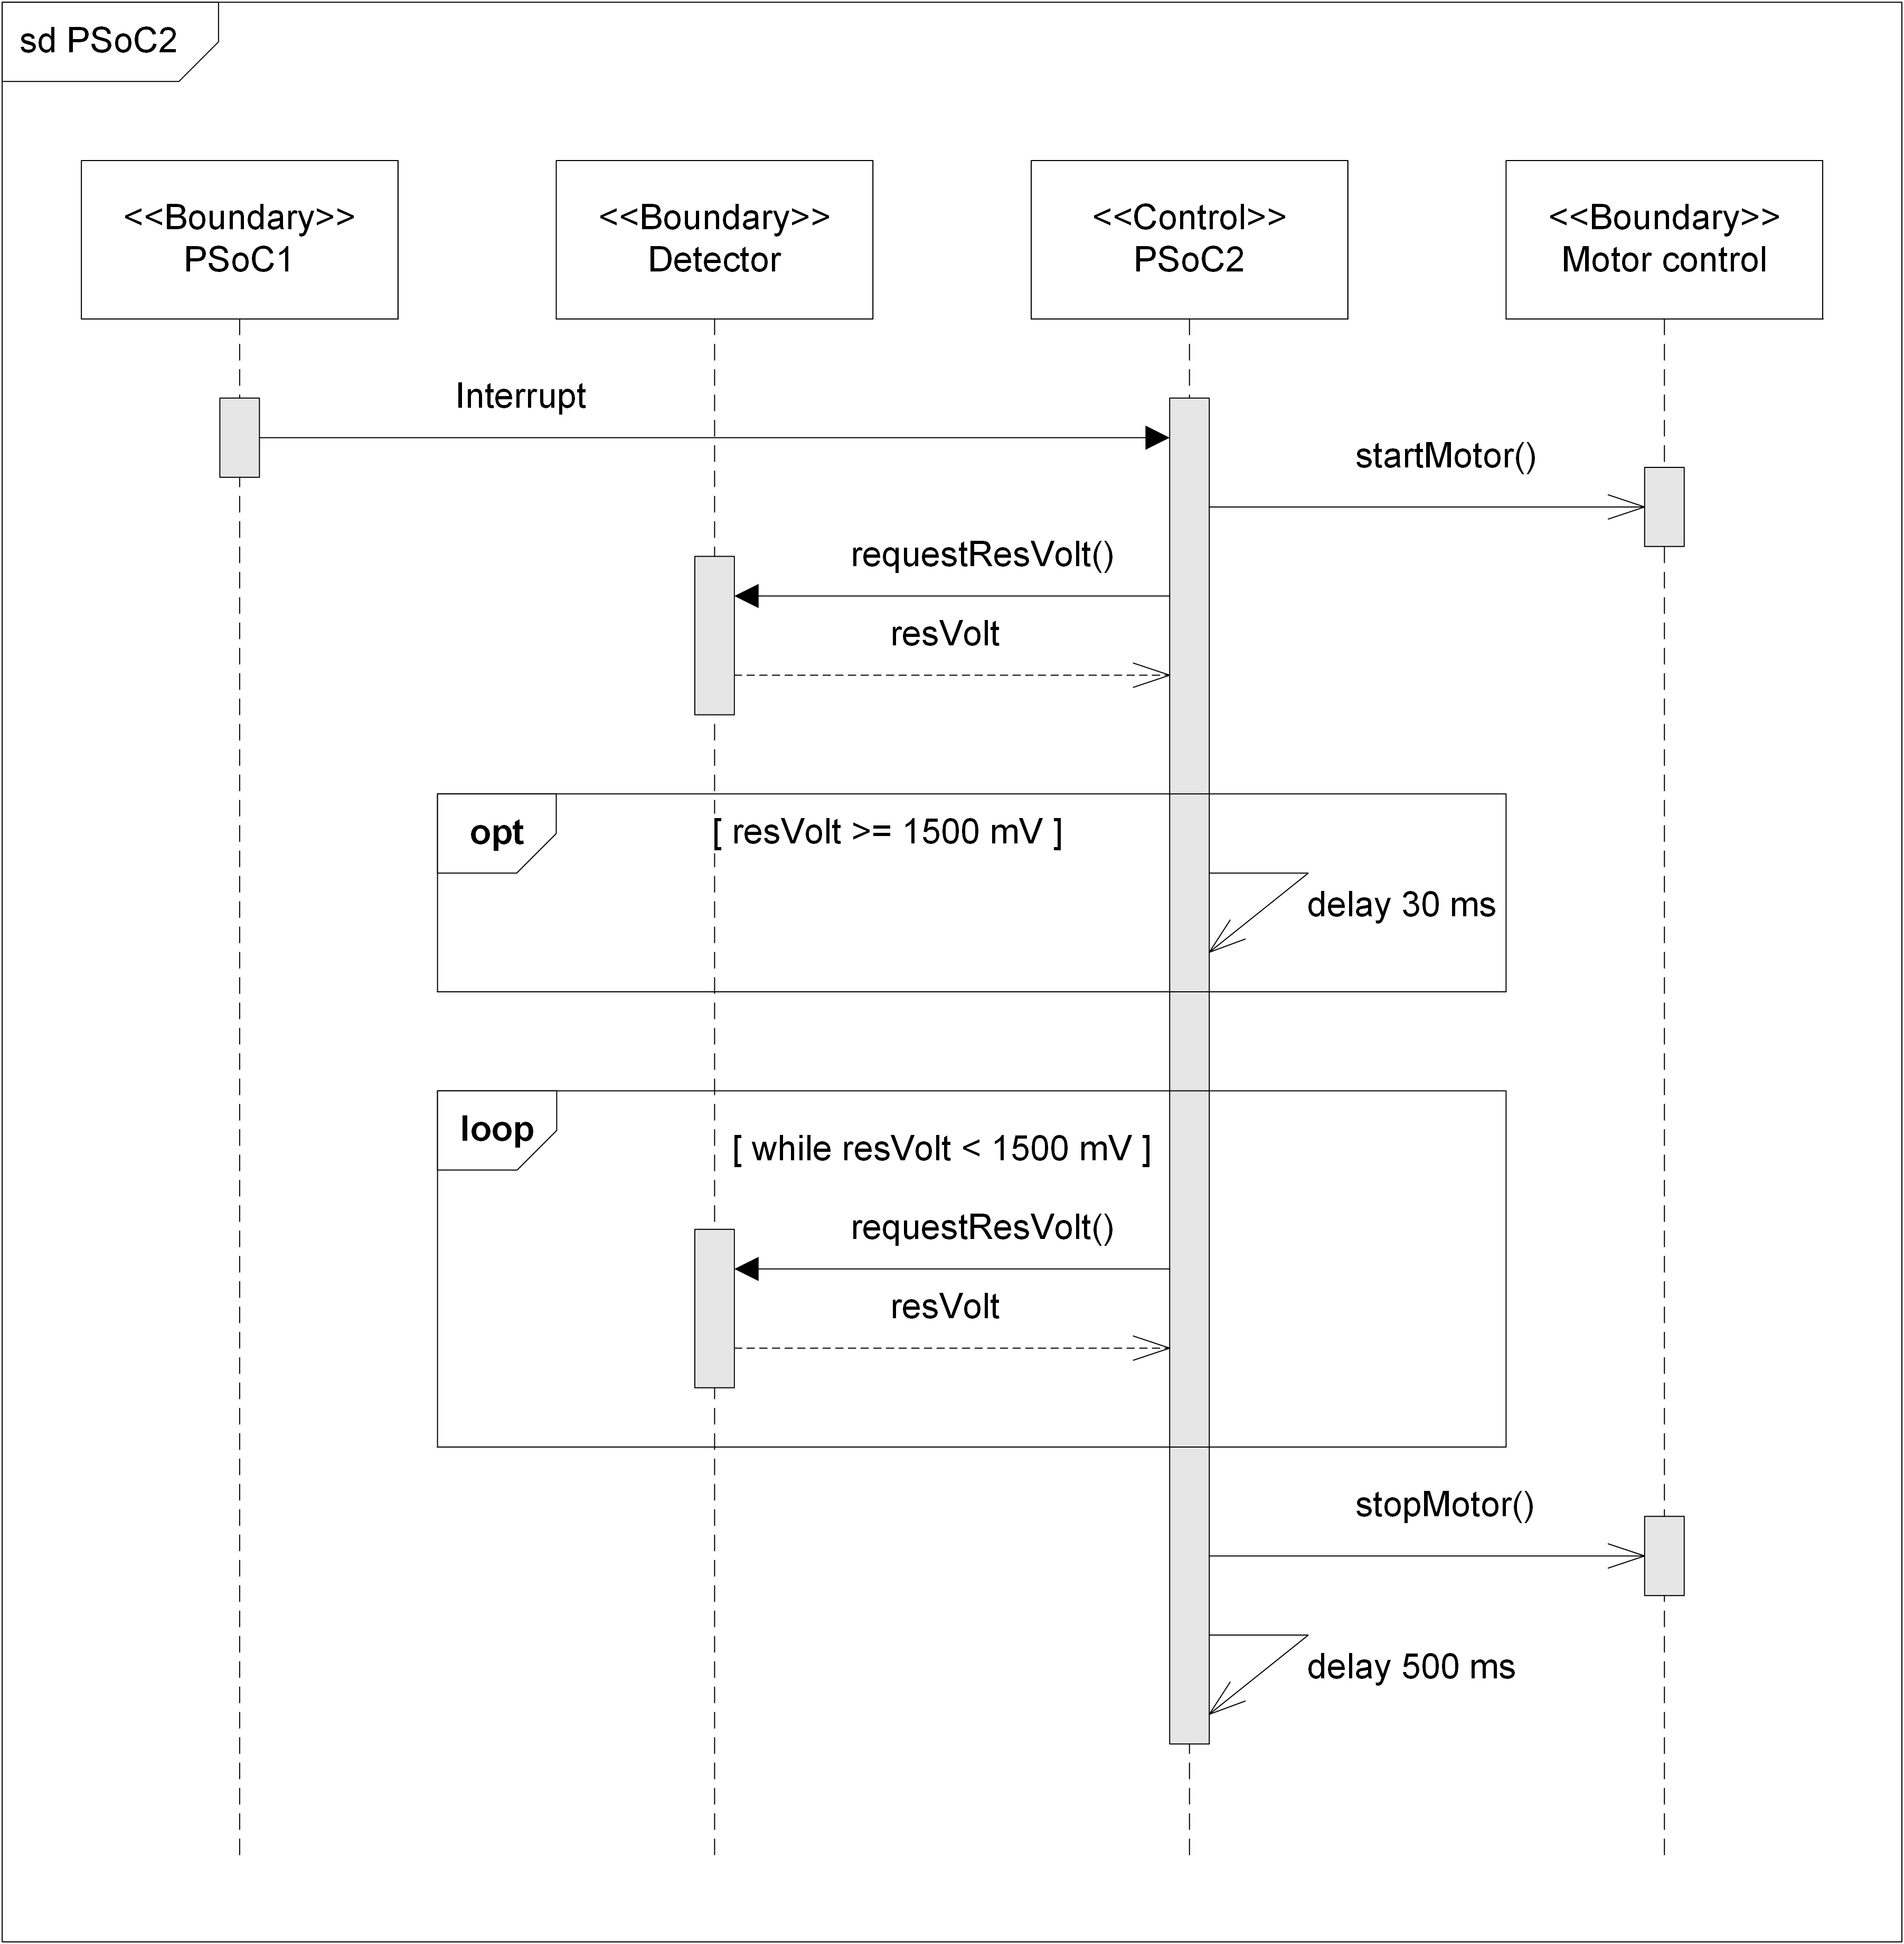
\includegraphics[width=1\textwidth]{Afsnit/DesignOgImplementering/images/PSoC2sekvens.png}
	\caption{Sekvensdiagram for PSoC2 software ved affyring af kanonen} %Jeg vil bare SÅ gerne have to interface drivere! :'(
	\label{fig:aktivitetsdiagramDetektor}
\end{figure}

Når der modtages et interrupt fra PSoC1, startes motoren, hvilket bevirker at kanonen begynder affyringen. Spændingen fra resVolt, anvendes til at vurdere, om fotodioden kan se lyset fra den røde LED. Normalt indikerer det, at de kan se hinanden, at affyringen er færdig, og at motoren skal stoppes, men hvis de kan se hinanden på dette tidspunkt ved interruptets start, betyder det, at de, inden affyringen er startet, allerede er placeret, så de kan se hinanden. Hvis det er tilfældet køres det delay, der ses i "opt-boksen" på figur \ref{fig:aktivitetsdiagramDetektor}. Det sker for at sikre, at motoren er drejet, så de igen ikke kan se hinanden. Derefter aflæses spændingen fra resVolt igen - nu for at tjekke om affyringen er afsluttet. Aflæsningen gentages indtil fotodioden kan se den røde LED, og motoren dermed skal stoppes. Til sidst er der indsat et delay på 500 ms, så der går et halvt sekund, inden der igen kan skydes. Derved undgås det, at kanonen affyres med det samme igen, hvis triggeren ved en fejl ikke er sluppet.